\documentclass[a4paper, 11pt]{article}
\usepackage{caption}
\captionsetup{tablename=Tabella}
\usepackage{slashbox}
\usepackage{pgfplots}
\pgfplotsset{/pgf/number format/use comma,compat=newest}

\begin{document}
\section*{Albero binario di ricerca (ABR) vs rosso-nero (ARN)}
\vspace{0,4 cm}

In questo esercizio si vuole mettere in risalto le differenza fra un albero binario di ricerca e uno rosso-nero.

\vspace{0,5 cm} 
Un albero binario di ricerca è una struttura dati composta da nodi identificati da chiavi univoche e legati fra loro da una relazione padre-figlio. Ogni nodo può avere un massimo di due figli: il figlio sinistro ha una chiave di valore minore rispetto a quella del padre, mentre il figlio destro ha una chiave di valore maggiore rispetto a quella del padre. Ogni albero ha una radice dalla quale si sviluppa e delle foglie che chiudono la struttura.
La forma della struttura dell'albero, che può essere diversa per lo stesso insieme di chiavi, dipende dall'ordine in cui i nodi sono inseriti al momento della costruzione.

\vspace{0,5 cm}
Un albero rosso-nero è un albero binario di ricerca in cui ogni nodo è corredato di un ulteriore attributo, il colore, il quale può assumere i valori rosso o nero. Ai nodi a cui mancano un figlio o un padre (nel caso della radice), si collega una sentinella (\textbf{T.NIL}) di colore nero, che quindi risulterà sempre come foglia della struttura. Inoltre, un albero rosso-nero, per essere tale, deve avere 5 proprietà:
\begin{enumerate}
\item Ogni nodo è rosso o nero
\item La radice è nera
\item Ogni foglia (\textbf{T.NIL}) è nera
\item Se un nodo è rosso, allora entrambi i suoi figli sono neri
\item Tutti i cammini da ogni nodo alle foglie contengono lo stesso numero di nodi
\end{enumerate}
La presenza di queste proprietà garantisce che ogni cammino che vada dalla radice alle foglie non sia lungo
più del doppio di qualsiasi altro cammino dalla radice alle foglie, rendendo così l'albero approssimativamente bilanciato.

\vspace{0,5 cm}
Per valutare la differenza fra le due tipologie di albero, sono stati svolti dei test nei quali si confronta l'altezza dei due alberi al variare del numero $n$ di nodi. Fra i test svolti sono presenti anche quelli nel caso peggiore, cioè quando l'array dal quale ricaviamo l'albero è ordinato (nei test svolti l'ordine è crescente).

\vspace{0,5 cm}
Dai risultati ci aspettiamo che l'altezza di un albero abbia un andamento \O$(log_2{n})$, questo perché ogni nodo può avere al massimo due figli. L'eccezione sarà nel caso peggiore dell'albero binario di ricerca, dove l'andamento dell'altezza deve corrispondere ad una retta di coefficiente 1, questo perché ogni nodo inserito durante la costruzione, è inserito come figlio destro del nodo precedentemente inserito.

\vspace{0,5 cm}
I test fatti sono basati su 4 dimensioni dell'albero (10, 100, 500, 1000 nodi). Per ogni dimensione sono stati svolti 10 run dei test, ognuno dei quali costruisce un albero partendo dall'array ordinato e altri 5 alberi basandosi sul rimescolamento dell'array originario.

\vspace{0,5 cm}
Sotto sono riportati i risultati:

\vspace{0,5 cm}
\begin{table}[h]
\footnotesize
\setlength{\tabcolsep}{5 pt}
\caption{Altezza albero binario di ricerca (ABR)}\label{etichetta}
\hspace{-3,5 cm}
\begin{tabular}{| c | c c c c c c | c c c c c c | c c c c c c | c c c c c c |}
\hline
\multicolumn{1}{| c |}{\backslashbox{Prova }{ N° nodi}}& \multicolumn{6}{| c |}{10} & \multicolumn{6}{| c |}{100} & \multicolumn{6}{| c |}{500} & \multicolumn{6}{| c |}{1000}\\
\hline
& \multicolumn{1}{| c |}{WC} & \multicolumn{1}{| c |}{1} & {2} & \multicolumn{1}{| c |}{3} & \multicolumn{1}{| c |}{4} & \multicolumn{1}{| c |}{5} & \multicolumn{1}{| c |}{WC} & \multicolumn{1}{| c |}{1} & {2} & \multicolumn{1}{| c |}{3} & \multicolumn{1}{| c |}{4} & \multicolumn{1}{| c |}{5} &\multicolumn{1}{| c |}{WC} & \multicolumn{1}{| c |}{1} & {2} & \multicolumn{1}{| c |}{3} & \multicolumn{1}{| c |}{4} & \multicolumn{1}{| c |}{5} &\multicolumn{1}{| c |}{WC} & \multicolumn{1}{| c |}{1} & {2} & \multicolumn{1}{| c |}{3} & \multicolumn{1}{| c |}{4} & \multicolumn{1}{| c |}{5}\\
\hline
1 & 10 & 5 & 5 & 7 & 6 & 5 & 100 & 12 & 14 & 14 & 18 & 12 & 500 & 18 & 20 & 19 & 17 & 20 & 1000 & 20 & 24 & 23 & 20 & 21\\
\hline
2 & 10 & 7 & 7 & 6 & 6 & 5 & 100 & 14 & 12 & 16 & 14 & 13 & 500 & 19 & 19 & 18 & 23 & 22 & 1000 & 26 & 23 & 23 & 24 & 21\\
\hline
3 & 10 & 5 & 5 & 5 & 7 & 6 & 100 & 13 & 16 & 13 & 11 & 17 & 500 & 19 & 18 & 18 & 21 & 23 & 1000 & 24 & 21 & 21 & 25 & 26\\
\hline
4 & 10 & 6 & 5 & 6 & 5 & 6 & 100 & 14 & 11 & 12 & 14 & 15 & 500 & 19 & 20 & 17 & 19 & 18 & 1000 & 19 & 25 & 21 & 23 & 24\\
\hline
5 & 10 & 5 & 6 & 6 & 7 & 5 & 100 & 12 & 12 & 14 & 12 & 13 & 500 & 18 & 18 & 18 & 18 & 19 & 1000 & 21 & 23 & 20 & 20 & 20\\
\hline
6 & 10 & 4 & 6 & 5 & 5 & 7 & 100 & 16 & 14 & 14 & 15 & 12 & 500 & 19 & 18 & 19 & 18 & 21 & 1000 & 24 & 24 & 24 & 23 & 23\\
\hline
7 & 10 & 6 & 5 & 7 & 5 & 6 & 100 & 13 & 13 & 14 & 13 & 13 & 500 & 22 & 17 & 21 & 18 & 20 & 1000 & 20 & 23 & 23 & 20 & 22\\
\hline
8 & 10 & 5 & 6 & 6 & 6 & 6 & 100 & 16 & 12 & 12 & 12 & 13 & 500 & 18 & 20 & 19 & 17 & 19 & 1000 & 23 & 22 & 23 & 20 & 27\\
\hline
9 & 10 & 5 & 6 & 7 & 6 & 6 & 100 & 13 & 14 & 15 & 13 & 14 & 500 & 16 & 21 & 20 & 19 & 21 & 1000 & 23 & 22 & 21 & 25 & 20\\
\hline
10 & 10 & 6 & 6 & 5 & 5 & 5 & 100 & 17 & 16 & 12 & 13 & 12 & 500 & 19 & 21 & 18 & 18 & 18 & 1000 & 21 & 22 & 20 & 24 & 20\\
\hline
\end{tabular}
\end{table}

\vspace{0,5 cm}
\begin{table}[h]
\footnotesize
\setlength{\tabcolsep}{5 pt}
\caption{Altezza albero rosso-nero (ARN)}
\hspace{-3,1 cm}
\begin{tabular}{| c | c c c c c c | c c c c c c | c c c c c c | c c c c c c |}
\hline
\multicolumn{1}{| c |}{\backslashbox{Prova }{ N° nodi}}& \multicolumn{6}{| c |}{10} & \multicolumn{6}{| c |}{100} & \multicolumn{6}{| c |}{500} & \multicolumn{6}{| c |}{1000}\\
\hline
& \multicolumn{1}{| c |}{WC} & \multicolumn{1}{| c |}{1} & {2} & \multicolumn{1}{| c |}{3} & \multicolumn{1}{| c |}{4} & \multicolumn{1}{| c |}{5} & \multicolumn{1}{| c |}{WC} & \multicolumn{1}{| c |}{1} & {2} & \multicolumn{1}{| c |}{3} & \multicolumn{1}{| c |}{4} & \multicolumn{1}{| c |}{5} &\multicolumn{1}{| c |}{WC} & \multicolumn{1}{| c |}{1} & {2} & \multicolumn{1}{| c |}{3} & \multicolumn{1}{| c |}{4} & \multicolumn{1}{| c |}{5} &\multicolumn{1}{| c |}{WC} & \multicolumn{1}{| c |}{1} & {2} & \multicolumn{1}{| c |}{3} & \multicolumn{1}{| c |}{4} & \multicolumn{1}{| c |}{5}\\
\hline
1 & 5 & 4 & 4 & 4 & 4 & 4 & 11 & 8 & 8 & 8 & 8 & 9 & 15 & 11 & 11 & 11 & 11 & 11 & 17 & 12 & 12 & 12 & 12 & 12\\
\hline
2 & 5 & 4 & 4 & 4 & 4 & 4 & 11 & 8 & 8 & 8 & 8 & 8 & 15 & 11 & 11 & 11 & 11 & 11 & 17 & 12 & 12 & 12 & 12 & 12\\
\hline
3 & 5 & 4 & 4 & 4 & 4 & 4 & 11 & 8 & 8 & 8 & 9 & 9 & 15 & 11 & 11 & 11 & 11 & 11 & 17 & 12 & 12 & 12 & 12 & 12\\
\hline
4 & 5 & 4 & 4 & 4 & 4 & 4 & 11 & 8 & 8 & 8 & 8 & 8 & 15 & 11 & 11 & 11 & 11 & 11 & 17 & 12 & 12 & 12 & 12 & 12\\
\hline
5 & 5 & 4 & 4 & 4 & 4 & 4 & 11 & 8 & 8 & 8 & 8 & 8 & 15 & 11 & 11 & 11 & 11 & 11 & 17 & 12 & 12 & 12 & 12 & 12\\
\hline
6 & 5 & 4 & 4 & 4 & 4 & 4 & 11 & 9 & 8 & 8 & 8 & 8 & 15 & 11 & 11 & 10 & 11 & 11 & 17 & 12 & 12 & 12 & 12 & 12\\
\hline
7 & 5 & 4 & 4 & 4 & 4 & 4 & 11 & 8 & 9 & 8 & 8 & 8 & 15 & 11 & 11 & 11 & 11 & 11 & 17 & 12 & 12 & 12 & 12 & 12\\
\hline
8 & 5 & 4 & 4 & 4 & 4 & 4 & 11 & 8 & 8 & 8 & 8 & 8 & 15 & 11 & 11 & 11 & 11 & 12 & 17 & 12 & 12 & 12 & 13 & 12\\
\hline
9 & 5 & 4 & 4 & 4 & 4 & 4 & 11 & 8 & 9 & 8 & 8 & 8 & 15 & 11 & 11 & 11 & 11 & 11 & 17 & 12 & 12 & 12 & 12 & 12\\
\hline
10 & 5 & 4 & 4 & 4 & 4 & 4 & 11 & 8 & 8 & 8 & 8 & 9 & 15 & 11 & 11 & 11 & 11 & 11 & 17 & 12 & 12 & 12 & 12 & 12\\
\hline
\end{tabular}
\end{table}
\newpage
\begin{center}
\begin{figure}
\centering
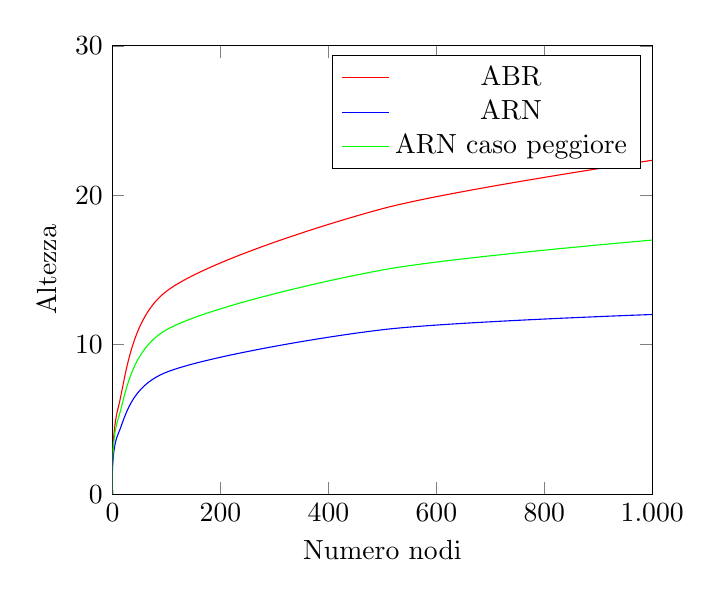
\begin{tikzpicture}
\begin{axis}[xmin=0, xmax=1000, ymin=0,ymax=30, xlabel=Numero nodi, ylabel=Altezza]
\addplot[smooth, red]
coordinates{(0,0) (10,5.72) (100,13.58) (500,19.1) (1000,22.34)};
\addplot[smooth, blue]
coordinates{(0,0) (10,4) (100,8.16) (500,11) (1000,12.02)};
\addplot[smooth, green]
coordinates{(0,0) (10,5) (100,11) (500,15) (1000,17)};
\legend{ABR,ARN,ARN caso peggiore}
\end{axis}
\end{tikzpicture}
\end{figure}
\end{center}

\vspace{1,5 cm}
Come ci si aspettava tutte le altezze hanno andamento logaritmico all'infuori del caso peggiore ABR, il quale ha un andamento lineare. E' stato scelto di non rappresentare il caso peggiore ABR nel diagramma cartesiano perché non avrebbe permesso di apprezzare la differenza fra gli andamenti delle altre altezze. Dal diagramma si nota che l' altezza dell'albero binario di ricerca è sempre maggiore a quella dell'albero rosso-nero, anche nel caso peggiore. La maggiore efficacia dell'ARN dipende dalla proprietà che la sua struttura è approssimativamente bilanciata. Il bilanciamento della struttura si può notare anche dai dati raccolti, i quali, a differenza di quelli dell'ABR, sono quasi del tutto omogenei.\\
L'ultima cosa da notare è per il caso peggiore (WC in tabella), che in entrambe le strutture mantiene gli stessi dati per ogni esecuzione dei test svolta sullo stesso numero di nodi. Questo è dovuto al fatto che, essendo l'array ordinato, le istruzioni svolte per la costruzione della struttura sono sempre le solite.
\newpage
\textbf{Documentazione codice}

\vspace{0,7 cm}
Il programma è stato scritto con Python nell'ambiente di sviluppo Pycharm.

\vspace{0,5 cm}
L'implementazione delle due strutture è stata possibile grazie all'uso di 4 classi implementate nel file \emph{abr\textunderscore{vs\textunderscore{arn}}}. \emph{Node} è la classe che permette di generare nodi per l'albero binario di ricerca. \emph{Abr} è la classe che genera alberi binari di ricerca al cui interno naturalmente ci sono nodi istanziati da \emph{Node}. La classe \emph{Arn}, la quale genera alberi rosso-nero, è composta da nodi istanziati dalla classe \emph{NodeArn}. La presenza di due classi diverse per la generazione di nodi è giustificata, oltre che dall'attributo colore, dagli attributi per il padre e per i figli. Infatti, mentre \emph{Node} immagazzina le chiavi dei nodi vicini, soluzione che snellisce il programma e la sua lettura, la classe \emph{NodeArn} immagazzina i nodi stessi. Quest'ultima scelta è dovuta alla presenza della sentinella, la quale essendo un vero e proprio nodo, ha bisogno di essere istanziata. Entrambe le classi che generano la struttura dati hanno come metodo interno \emph{height}, che calcola l'altezza del relativo albero.

\vspace{0,5 cm}
Nel file \emph{test\textunderscore{abr\textunderscore{vs\textunderscore{arn}}}} sono stati svolti, tramite \emph{unittest}, i test di cui sopra sono riportati i dati. La classe che implementa i test si chiama \emph{TestCase}, e tramite la funzione di setUp() permette ad ogni esecuzione di generare 5 array con ordine casuale e 1 ordinato, da cui vengono poi creati i rispettivi alberi.
\end{document}